% =============================================================================
% LaTeX Template for Academic and Professional Documents
% Author: Nicolas Huber
% Email: nicolas.huber2@uzh.ch
% 
% This template is created for academic and professional use. 
% Feel free to customize it to fit your needs. Attribution is appreciated but not required.
% =============================================================================

\documentclass[12pt]{article}

% --- Packages Start ---
\usepackage[a4paper]{geometry} % Geometry and layout
\usepackage{amsmath,amssymb,amsfonts} % Fonts and symbols
\usepackage{zi4} % Nice font for listings
\usepackage{graphicx} % Graphics and figures
\usepackage{float} % Improved interface for floating objects
\usepackage{listings} % Code listings
\usepackage{cite} % Bibliography
\usepackage{enumitem} % Customized lists
\usepackage{algorithmic} % Algorithms
\usepackage{textcomp} % Additional text symbols
\usepackage{xcolor} % Custom color support
\usepackage{booktabs} % Publication quality tables
% --- Packages End ---

% --- Custom Commands Start ---
\newcommand{\ie}{\textit{i.e., }}
\newcommand{\eg}{\textit{e.g., }}
\newcommand{\etal}{\textit{et al. }}
\newcommand{\cf}{\textit{cf. }}
\newcommand{\til}{\char`\~}
% --- Custom Commands End ---

% --- Custom Colors Start ---
\definecolor{deepblue}{rgb}{0,0,0.5}
\definecolor{deepred}{rgb}{0.6,0,0}
\definecolor{deepgreen}{rgb}{0,0.5,0}
% --- Custom Colors End ---


% --- Custom Listing Start ---
\lstset{
  basicstyle=\ttfamily\small,
  commentstyle=\color{deepgreen},
  keywordstyle=\color{deepblue},
  stringstyle=\color{deepred},
  showstringspaces=false,
  frame=none, % can be single
  numbers=left,
  numberstyle=\tiny\color{gray},
  breaklines=true,
  postbreak=\mbox{\textcolor{red}{$\hookrightarrow$}\space},
}

\lstdefinestyle{bashstyle}{
  language=bash,
  backgroundcolor=\color{gray!10}, % Light gray background
  morekeywords={dstat, --output},
}

\lstdefinestyle{pythonstyle}{
  language=Python,
  backgroundcolor=\color{gray!10}, % Light gray background
  morekeywords={def, return, if, else, print},
}
% --- Custom Listing End ---

\begin{document}

\begin{titlepage}
    \centering
    \vspace*{1cm}
    \Huge
    \textbf{Course Name}\\
    \vspace{0.5cm}
    \LARGE
    Course Number: XXXX\\
    \vspace{1.5cm}
    \textbf{Assignment Number: XX}\\
    \vspace{2cm}
    \textbf{University of Technology Sydney}\\
    \vfill
    
\includegraphics[width=0.4\textwidth]{assets/images/uts-logo.png}\\
    \vfill
    \Large
    Author Names\\
    Student ID: XXXXXX\\
    Date: \today
\end{titlepage}

\pagenumbering{roman}
\tableofcontents
\newpage

\pagenumbering{arabic}
\section{Introduction}
\subsection{Background}

This is a sentence with a ref~\cite{Aydeger2019UtilizingAttacks}.


\begin{figure}[H]
    \centering
    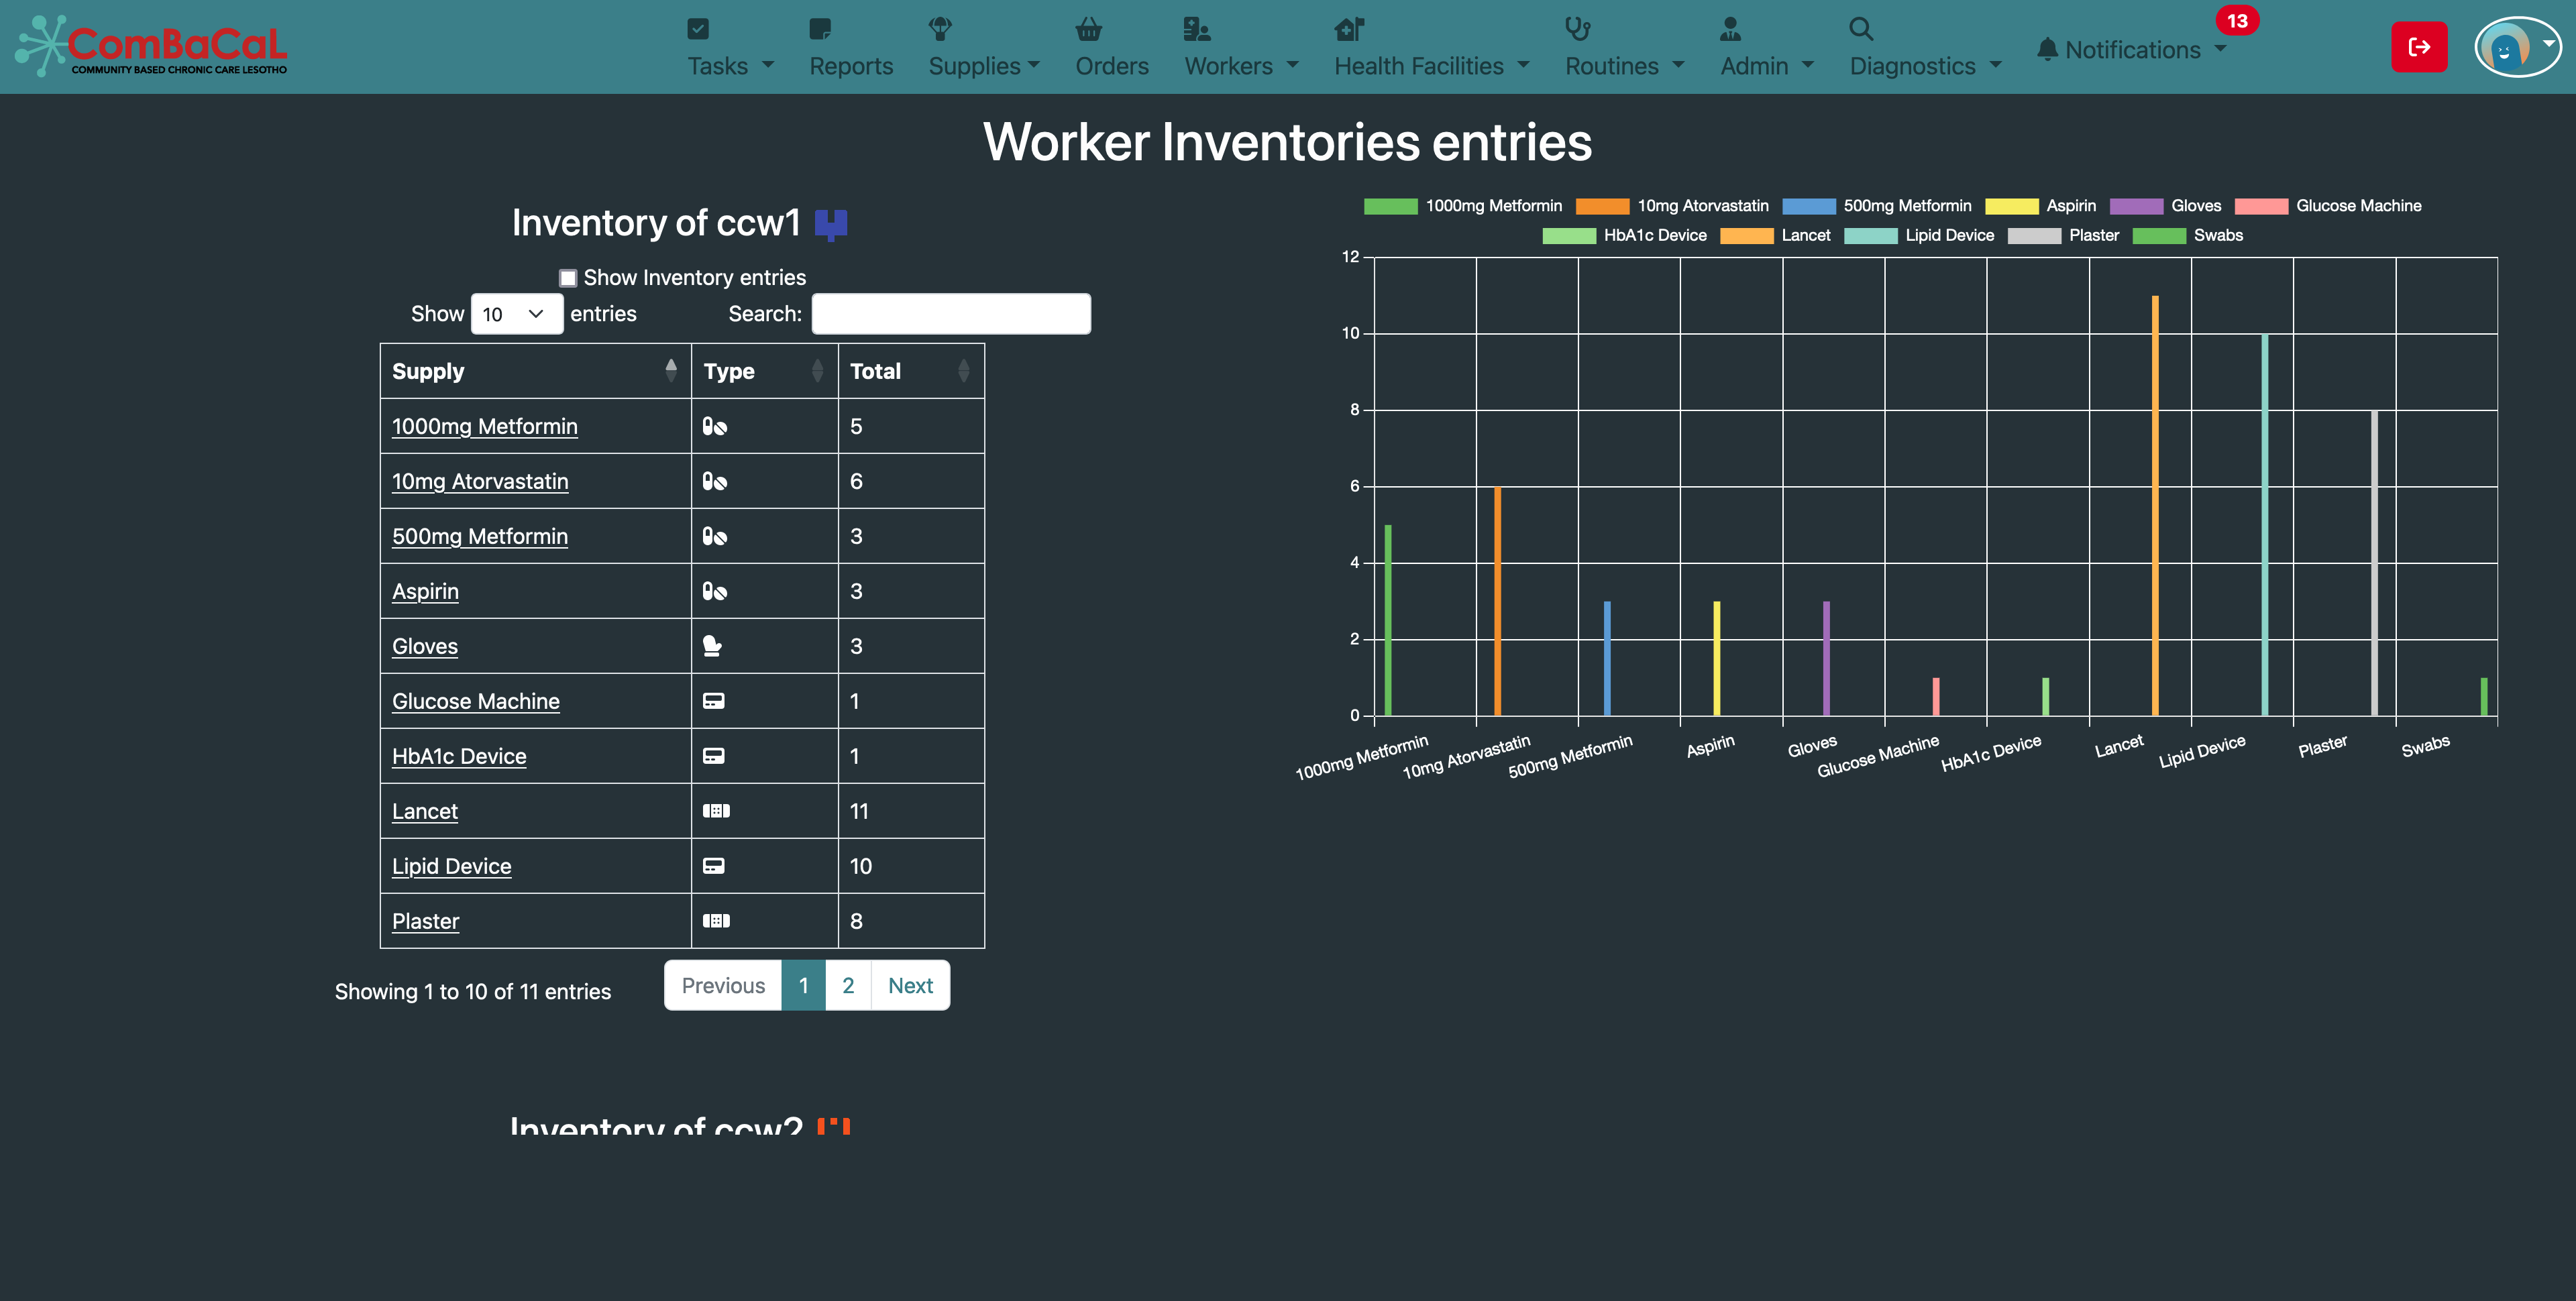
\includegraphics[trim=0cm 10cm 0.0cm 0cm, clip, width=\linewidth]{assets/images/admin-panel-32-worker-inventories-synced.png}
    \caption{Selection Framework Optimizing Four MTD Techniques}
    \label{fig:architecture}
\end{figure}


\begin{lstlisting}[caption={Measuring System Impact of the Dynamic Analysis using\textit{dstat}},label=measurement]
dstat -t --cpu --mem --fs -d --disk-tps 
      -n --tcp --socket -y -p -N eth0 
      --output $filename $delay $observations
\end{lstlisting}

\begin{lstlisting}[language=Python,caption={Python code to calculate the factorial of a number.}]
# Function to calculate the factorial of a number
def factorial(n):
    """Calculate the factorial of a number n"""
    if n == 0:
        return 1
    else:
        return n * factorial(n-1)

# Calling the factorial function
number = 5
result = factorial(number)
print(f"The factorial of {number} is {result}")
\end{lstlisting}


\begin{table}
    \centering
    \caption{Detection time}\label{table:evaluation-detection-time}
    \scriptsize
    \begin{tabular}{lllllll}
        \hline
        & \multicolumn{3}{l|}{Trigger point} & \multicolumn{1}{l|}{} & Time interval & \\
        & \textbf{Malware} & \textbf{Download} & \multicolumn{1}{l|}{\textbf{MTD}} & \multicolumn{1}{l|}{\textbf{MTD}} & \textbf{Detection (s)} & \textbf{Deployment (s)} \\
        \hline
        "Ransomware-PoC" & 07:15:00 & - & 07:15:26 & 1 & 26 & 143.78 \\
        "httpBackdoor" & 07:26:00 & - & 07:26:26 & 2 & 26 & 8.94 \\
        "BEURK" & 07:38:00 & - & 07:38:04 & 3 & 4 & 0.3 \\
        "The Tick" & 07:52:00 & 07:50:30 & 07:52:34 & 4 & 124 (154) & 9.01 \\
        "backdoor" & 08:10:00 & 08:10:30 & 08:10:38 & 4 & 8 (38) & 9.02 \\
        "bdvl" & 08:22:00 & - & 08:22:04 & 3 & 4 & 0.25s \\
        "BASHLITE" & 08:32:00 & - & - & - & - & - \\
        \hline
    \end{tabular}
\end{table}


\subsection{Objective}

\section{Methodology}



\bibliographystyle{IEEEtran}
\bibliography{references}

\end{document}
